\documentclass{beamer}
%
% Choose how your presentation looks.
%
% For more themes, color themes and font themes, see:
% http://deic.uab.es/~iblanes/beamer_gallery/index_by_theme.html
%
\mode<presentation>
{
  \usetheme{default}      % or try Darmstadt, Madrid, Warsaw, ...
  \usecolortheme{default} % or try albatross, beaver, crane, ...
  \usefonttheme{default}  % or try serif, structurebold, ...
  \setbeamertemplate{navigation symbols}{}
  \setbeamertemplate{caption}[numbered]
  \setbeamertemplate{footline}[frame number]
} 

\usepackage[english]{babel}
\usepackage[utf8]{inputenc}
\usepackage[T1]{fontenc}
\usepackage{hyperref}
\usepackage{listings}
\usepackage{minted}

\title[Your Short Title]{Introduction to R}
\author{Fusheng Yang}
\institute{Department of Statistics, University of Connecticut}
\date{October 8, 2022}

\begin{document}

\begin{frame}
  \titlepage
\end{frame}

% Uncomment these lines for an automatically generated outline.
%\begin{frame}{Outline}
%  \tableofcontents
%\end{frame}

\section{Welcome}

\begin{frame}{Welcome}

\begin{itemize}
  \item This workshop is a part of \href{https://statds.org/events/ucsas2022/index.html}{UCONN SPORTS ANALYTICS SYMPOSIUM (UCSAS) 2022}
  \item This workshop aims to give a quick tour of R
  \item All source codes of related documents of this workshop are in the GitHub repository: \url{https://github.com/fushengyy/UCSAS2022_intro_to_R}
  
\end{itemize}

\end{frame}

\section{About Me}

\begin{frame}{About Me}

\begin{itemize}
  \item Fourth-year Ph.D. Student in Statistcs at UConn.
  \item Research Interests: 
  \begin{itemize}
      \item Time series analysis and extreme value analysis.
  \end{itemize}
  \item Future goals:
  \begin{itemize}
      \item Contribute to the broader field of environmental statistics.
  \end{itemize}
\end{itemize}

\end{frame}


\section{Prerequisites}

\begin{frame}{Prerequisites}

\begin{itemize}
    \item A laptop with R/RStudio installed.
    \begin{itemize}
        \item R can be downloaded for windows users \href{https://cran.r-project.org/bin/windows/base/}{here} and for Mac users \href{https://cran.r-project.org/bin/macosx/}{here}
        \item RStudio can be downloaded for all users \href{https://www.rstudio.com/products/rstudio/download/}{here}
    \end{itemize}
    \item Little to no experience with R.
\end{itemize}
    
\end{frame}

\section{Outline}

\begin{frame}{Outline}
    
\begin{itemize}
    \item R Basics
    \item R Data Structure
    \item Read and Write Data
    \item Data Management
    \item Brief Overview of "dplyr" Package
\end{itemize}
    
\end{frame}

\section{What is R?}

\begin{frame}{What is R?}
    \begin{itemize}
        \item R is a free and open-source language and environment for statistical computing and graphics.
        \item First created by statisticians Ross Ihaka and Robert Gentleman in August 1993.
        \item Now supported by the R Core Team (formed in 1997) and the R Foundation for Statistical Computing (formed in 2003).
    \end{itemize}
\end{frame}

\section{What is RStudio?}

\begin{frame}{What is RStudio?}
    \begin{itemize}
        \item RStudio is an integrated development environment (IDE) for R.
        \item It is available in two formats:
        \begin{itemize}
            \item \textbf{RStudio Desktop}: a regular desktop application
            \item RStudio Server: runs on a remote server and allows accessing RStudio using a web browser
        \end{itemize}
    \end{itemize}
\end{frame}

\section{RStudio Interface}

\begin{frame}{RStudio Interface}
    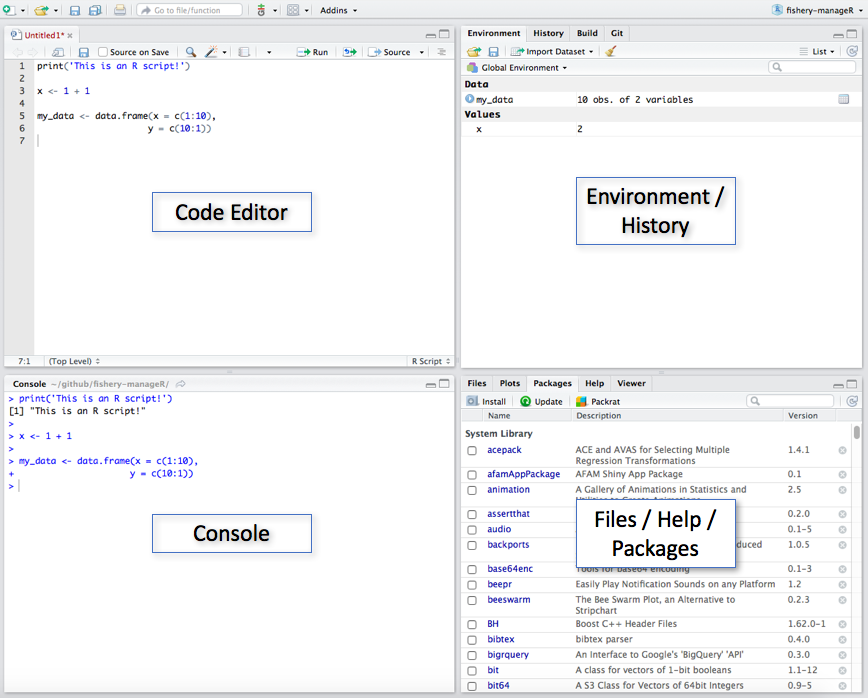
\includegraphics[scale = 0.425]{rstudio_ide_1.png}
\end{frame}

\section{R Basics}

\subsection{R as a Calculator}
\begin{frame}{R as a Calculator}
$+$ Addition\\
$-$ Subtraction\\
$*$ Multiplication\\
$/$ Division\\
$\wedge$ or $**$ Exponentiation\\
\hfill


Some built-in functions:\\
\texttt{sqrt()} Square root\\
\texttt{log()} Natural log\\
More \href{https://www.javatpoint.com/r-built-in-functions}{here}\\
\hfill

Example:\\
\texttt{3+8}\\
\texttt{exp(3)}\\
\texttt{sqrt(9)}
\end{frame}

\subsection{Getting Help}
\begin{frame}{Getting Help}

The \texttt{help()} function and \texttt{?} operator in R provide access to the documentation pages for R functions, data sets, and other objects.\\
\hfill

Example:\\
To get help with the \texttt{mean} function, we can use either
\texttt{help(mean)}
or 
\texttt{?mean}
    
\end{frame}

\subsection{Assignment Operators}

\begin{frame}{Assignment Operators}
Assign a value to a name using \texttt{<-}, \texttt{->}, or \texttt{=}.\\
\hfill

Example:\\
\texttt{x <- 5}\\
\texttt{"Hello World!" -> y}\\
\texttt{z = 2022}
\end{frame}

\section{R Data Structure}

\subsection{Data Types}

\begin{frame}{Data Types}
    In R, there are 6 basic data types:
    \begin{itemize}
        \item Logical: boolean data type, can have two values: \texttt{TRUE} and \texttt{FALSE}.
        \item Numeric: all real numbers with or without decimal values.
        \item Integer: real values without decimal points
        \item Complex: purely imaginary values
        \item Character: character or string values. 'A' is a single character, "Apple" is a string. You can use single quotes '' or double quotes "".
        \item Raw: specifies values as raw bytes. This will NOT be discussed in this workshop.
    \end{itemize}
\end{frame}

\subsection{Data Structures}

\begin{frame}{Data Structures}
R has many data structure. The most essential ones are
\begin{itemize}
    \item Vector
    \item List
    \item Dataframe
    \item Matrix
    \item Array
    \item Factor
\end{itemize}
    
\end{frame}

\begin{frame}{Data Structures (cont.)}
\begin{itemize}
    \item Vector: a collection of elements. Note the elements of a vector must be of the identical data type (Homogeneous). Vectors are one-dimensional data structures.
    \item List
    \item Dataframe
    \item Matrix
    \item Array
    \item Factor
\end{itemize}
    
\end{frame}

\begin{frame}{Data Structures (cont.)}
\begin{itemize}
    \item Vectors
    \item List: a generic object consisting of an ordered collection of objects. A list can contain vectors or elements of unequal dimensions or different data types (Heterogeneous).
    \item Dataframe
    \item Matrix
    \item Array
    \item Factor
\end{itemize}
    
\end{frame}

\begin{frame}{Data Structures (cont.)}
\begin{itemize}
    \item Vector
    \item List
    \item Dataframe: generic data objects of R which are used to store the tabular data. Dataframes are two-dimensional, heterogeneous data structures contain lists of vectors of equal lengths. Note a dataframe must have column names. Each column must have the identical number of items. Each item in a single column must be of the same data type. Different columns may have different data types.
    \item Matrix
    \item Array
    \item Factor
\end{itemize}
    
\end{frame}

\begin{frame}{Data Structures (cont.)}
\begin{itemize}
    \item Vector
    \item List
    \item Dataframe
    \item Matrix: a rectangular arrangement of numbers in rows and columns. Matrices are two-dimensional, homogeneous data structures.
    \item Array
    \item Factor
\end{itemize}
    
\end{frame}

\begin{frame}{Data Structures (cont.)}
\begin{itemize}
    \item Vector
    \item List
    \item Dataframe
    \item Matrix
    \item Array: the R data objects which store the data in more than two dimensions. Arrays are n-dimensional data structures.
    \item Factor
\end{itemize}
    
\end{frame}

\begin{frame}{Data Structures (cont.)}
\begin{itemize}
    \item Vector
    \item List
    \item Dataframe
    \item Matrix
    \item Array
    \item Factor: the data objects which are used to categorize the data and store it as levels. They are useful for storing categorical data.
\end{itemize}
    
\end{frame}

\begin{frame}{Data Structures (cont.)}
\begin{table}[]
\begin{tabular}{lll}
   & Homogeneous & Heterogeneous \\ \hline
1d & Vector     & List         \\ \hline
2d & Matrx   & Dataframe    \\ \hline
nd & Array       &              
\end{tabular}
\end{table}
    
\end{frame}

\begin{frame}{Quiz 1}
    Consider $x = (7,7,9,6,55,2)$\\
    \begin{itemize}
        \item What is the length of this vector?
        \item What are unique values of $x$?
        \item Sort the values of $x$.
        \item Frequency distribution of $x$.
    \end{itemize}
\end{frame}

\begin{frame}{Quiz 2}
How would you describe the following three objects? What makes them different to 1:5?\\
\hfill

\texttt{x1 <- array(1:5, c(1, 1, 5))}\\
\texttt{x2 <- array(1:5, c(1, 5, 1))}\\
\texttt{x2 <- array(1:5, c(1, 5, 1))}
\end{frame}

\begin{frame}{Quiz 3}
Let $A = \begin{bmatrix}
    1 & 2 \\
    3 & 4
  \end{bmatrix}$
and $B = \begin{bmatrix}
    5 & 7 \\
    6 & 8
  \end{bmatrix}$\\
\hfill

Find\\
\begin{itemize}
    \item dimensions of $A$ and $B$;
    \item determinants of $A$ and $B$;
    \item $A+B$;
    \item $AB$;
    \item $A^{-1}$ and $B^{-1}$.
\end{itemize}

\end{frame}

\subsection{Function}

\begin{frame}[fragile]{Function}
- An R function is created by using the keyword "function".\\
\hfill

- Basic syntax:
\begin{lstlisting}[language=R]
function_name <- function(arg_1, arg_2, ...) {
    Function body
}
\end{lstlisting}\\
\hfill

- Components:\\
\textit{Function Name}: the actual name of the function. It is stored in R environment as an object with this name.\\
\textit{Arguments}: a placeholder. When a function is invoked, you pass a value to the argument. Arguments are optional; that is, a function may contain no arguments. Also arguments can have default values.\\
\textit{Function Body}: contains a collection of statements that defines what the function does.\\
\textit{Return Value}: the last expression in the function body to be evaluated.

\end{frame}

\begin{frame}{Quiz 4}
    Write a function that takes $x$ and $y$ as inputs and returns the value $y^x$.
\end{frame}

\subsection{Loop and Condition}

\begin{frame}{Loop}
We use loop to deal with repeated tasks.\\
\hfill

- \textbf{for} loop: the most commonly used loop structure when you want to repeat a task a defined number of times.

- \textbf{while} loop: used when you want to keep looping until a specific logical condition is satisfied (contrast this with the for loop which will always iterate through an entire sequence).

\end{frame}

\begin{frame}{Condition}

- \textbf{if} Statement: The \textit{if} statement takes a condition; if the condition evaluates to \textit{TRUE}, the R code associated with the \textit{if} statement is executed.

- \textbf{if ... else ...} Statement: The code associated with the \textit{else} statement gets executed whenever the condition of the \textit{if} condition is \textit{FALSE}.

- \textbf{if ... else if ... else} Statement: The \textit{else if} condition is checked if the first condition is not satisfied. If the second condition is then met, then the code inside it is executed.

\end{frame}

\begin{frame}{Quiz 5}
Using the conditional statement, check whether -9 is divisible by 2 or by 3.
\end{frame}

\section{Read and Write Data}

\subsection{Local Directory}

\begin{frame}[fragile]{Read and Write Data from/to Local Directory}
- Read data syntax:
\begin{lstlisting}[language=R]
read.table(file = "location_of_file", 
           header = TRUE)
\end{lstlisting}\\

- Write/Save data syntax:
\begin{lstlisting}[language=R]
write.table(dataName, 
            file = "location_of_file")
\end{lstlisting}\\

- Some useful functions:
\begin{lstlisting}[language=R]
read.csv(), read.csv2(), 
write.csv(), write.csv2(), 
etc.
\end{lstlisting}\\

\end{frame}

\subsection{Packages}

\begin{frame}[fragile]{Install and Load R Packages}
- Install a package syntax:
\begin{lstlisting}[language=R]
install.packages("package_name")
\end{lstlisting}\\

- Load a package syntax:
\begin{lstlisting}[language=R]
library("package_name")
\end{lstlisting}\\

- Install and load "Lahman" package:
\begin{lstlisting}[language=R]
install.packages("Lahman")
library(Lahman)
\end{lstlisting}\\

"Lahman" package contains historical season-level baseball data for Major League Baseball going back to 1871.
    
\end{frame}

\begin{frame}[fragile]{Search and Read Datasets in a Package}
- Search datasets from a package syntax:
\begin{lstlisting}[language=R]
data(package = "package_name")
\end{lstlisting}\\

- Read a particular dataset from a package syntax:
\begin{lstlisting}[language=R]
data("dataName", package = "package_name")
\end{lstlisting}
\end{frame}

\begin{frame}{Dataframe}
\texttt{str(Batting)}: Learn more about variables. For more information check \href{https://rdrr.io/cran/Lahman/man/Batting.html}{here}.\\
\texttt{names(Batting)}: Names of the dataset.\\
\texttt{head(Batting)}: Display the first few rows of the dataset.\\
\texttt{Batting[, 1:4]}: Display the first 4 columns of the dataset.\\
\texttt{Batting[1:4,]}: Display the first 4 rows of the dataset.\\
\texttt{Batting\$playerID}: Display values of the variable "playerID".\\
\texttt{Batting[, c("playerID")]}: Display values of the variable "playerID".\\
\texttt{Batting[1:10, c("playerID", "yearID")]}: Display the first 10 elements of the variables "playerID" and "yearID".\\
\texttt{Batting\$CS\_SO <- Batting\$CS + Batting\$SO}: Create a new variable "CS\_SO" by adding up values of variables "CS" and "SO".\\
\texttt{Batting[, c("CS", "SO", "CS\_SO")]}: Display only "CS", "SO", and "CS\_SO" of the updated dataset
\end{frame}

\begin{frame}{Quiz 6}
Using Batting dataset
\begin{itemize}
    \item Display data from year 1900 only.
    \item Find total number of players and teams played through out all games in the dataset.
    \item Create a new dataframe "Batting1950" for year 1950 only.
\end{itemize}
\end{frame}

\section{dplyr}

\begin{frame}{Data Manipulation using dplyr}
dplyr: an R package which provides a set of tools for efficiently manipulating datasets.
    
\end{frame}

\begin{frame}[fragile]{Data Manipulation using dplyr (cont.)}
- Installation and loading:
\begin{lstlisting}[language=R]
install.packages("dplyr")
library(dplyr)
\end{lstlisting}

- Load dataset "Salaries" from package "Lahman":
\begin{lstlisting}[language=R]
data("Salaries", package = "Lahman")
head(Salaries)
\end{lstlisting}
\end{frame}

\begin{frame}[fragile]{Data Manipulation using dplyr (cont.)}
- Remove league info (variable "lgID") from "Salaries". i.e. select all variables but "lgID":
\begin{lstlisting}[language=R]
salaries <- Salaries %>%
             select(playerID, yearID, 
                    teamID, salary)
head(salaries)
\end{lstlisting}

- Join salary info and batting info together:
\begin{lstlisting}[language=R]
batting <- left_join(Batting, salaries, 
                by = c("playerID", "yearID", 
                       "teamID"))
head(batting)
\end{lstlisting}

\texttt{left\_join(a, b, by = "x1")}: Join matching rows from b to a.\\
More join options check \href{https://www.rstudio.com/wp-content\%2Fuploads\%2F2015\%2F02\%2Fdata-wrangling-cheatsheet.pdf\%2F}{here}.

- Rearrange orders of the dataset by multiple variables:
\begin{lstlisting}[language=R]
batting <- batting %>% arrange(playerID, yearID)
\end{lstlisting}

\end{frame}

\begin{frame}{Quiz 7}

\begin{itemize}
    \item Using "Batting" dataset to find players who have a minimum of 25 base on balls before the year of 1900 and save to a new dataframe "player25".
    \item Rearrange these players based on base on balls in a descending order and save to a new dataframe "player25\_ordered".
\end{itemize}
\end{frame}

\section{Reference}

\begin{frame}{Useful References}
\begin{itemize}
    \item \href{https://bookdown.org/rdpeng/rprogdatascience/}{R Programming for Data Science} by Roger D. Peng
    \item \href{https://cran.r-project.org/doc/manuals/r-release/R-intro.pdf}{An Introduction to R} by W. N. Venables, D. M. Smith and the R Core Team
    \item \href{https://r4ds.had.co.nz/index.html}{R for Data Science} by Hadley Wickham and Garrett Grolemund
\end{itemize}
\end{frame}

\begin{frame}{}
\centering \Huge
\emph{Thank You!}
\end{frame}


\end{document}
